%! TeX program = lualatex
%! TeX root = main.tex

\def\basedir{/home/theammir/labs/oop}
%! TeX program = lualatex
\documentclass[a4paper,14pt]{extarticle}
\usepackage[left=2.5cm,right=1.5cm,
		top=2cm,bottom=2cm,bindingoffset=0cm]{geometry}
\usepackage{fontspec}
\usepackage{fancyhdr}
\usepackage{fancyvrb}
\setmainfont{FreeSerif}
\setmonofont{FiraCode}
\usepackage[english,ukrainian]{babel}
\usepackage[position=bottom]{caption}

\usepackage{minted}
\setminted{style=arduino}
\setminted{mathescape}

\usepackage{caption}
\captionsetup[listing]{name=Файл}

\pagestyle{fancy}
\fancyhead{}
\fancyfoot[C]{}
\fancyfoot[R]{\thepage}
\setlength{\headheight}{17pt}
\renewcommand{\headrulewidth}{0pt}

\setcounter{secnumdepth}0

\newcommand{\shell}[2][build/temp.tex]{%
	\immediate\write18{#2 > #1}%
	\CatchFileDef{\out}{#1}{\endlinechar=13}%
}

\newcommand{\codefile}[2]{%
	\begin{center}
		\inputminted[tabsize=2, breaklines, fontsize=\small]{#1}{\basedir/\thelabid/#2}
		\captionof{listing}{\detokenize{#2}}
	\end{center}
}

\newcommand{\thetitlepage}[4]{
	\def\thelabno{#1}
	\def\thelabid{\thelabno}
	\def\thestudentno{#4}
	
	\begin{titlepage}
	\begin{center}
		\vspace{1cm}
		\textbf{Міністерство освіти і науки України\\
		Національний технічний університет України\\
		<<Київський політехнічний інститут імені Ігоря Сікорського>>\\
		Факультет інформатики та обчислювальної техніки\\
		Кафедра обчислювальної техніки\\}
		\vspace*{5cm}
		\textbf{Лабораторна робота №#1\\}
		\vspace{0.5cm}
		з дисціпліни\\
		<<Об'єктно-орієнтоване програмування>>
		\vspace*{7cm}
		
		\begin{tabular}{ll}
		\begin{minipage}[t]{0.54\linewidth}
			Виконав:\\
			студент групи #2\\
			#3\\
			номер у списку групи: \thestudentno\par
		\end{minipage}
		&
		\begin{minipage}[t]{0.3\linewidth}
			Перевірив:\\
			Порєв В.~М.
		\end{minipage}
		\end{tabular}

		\vfill
		Київ \the\year\\
	\end{center}
	\end{titlepage}
	\setcounter{page}2
}

\newcommand{\taskdesc}{\section*{Завдання}}

\newcommand{\taskspec}{\section{Варіант \thestudentno}}

\newcommand{\codetext}{\section{Текст програм}}

\newcommand{\tasktest}{\section{Результати тестування програми}}

\newcommand{\conclusion}{\section{Висновок}}

% vim: ts=2: sw=2


\usepackage{graphicx}

\begin{document}
\thetitlepage{1}{ІМ-42}{Туров Андрій Володимирович}{26}
\def\thelabid{lab1}

\taskspec%
Завдання 2 + 3:
\begin{enumerate}
	\setcounter{enumi}{1}
	\item Два вікна діалогу. Спочатку з’являється перше, яке має дві кнопки: [Далі >]
		і [Відміна]. Якщо натиснути кнопку [Далі >], то воно закриється і з’явиться
		друге діалогове вікно, яке має кнопки: [< Назад], [Так] і [Відміна]. Якщо натиснути
		кнопку [<Назад], вікно закриється і перехід до першого вікна.
	\item Вікно діалогу з елементом списку (List Box) та двома кнопками: [Так] і
		[Відміна]. У список автоматично записуються назви груп нашого факультету. Якщо
		вибрати потрібний рядок списку і натиснути [Так], то у головному вікні повинен
		відображатися текст вибраного рядка списку.
\end{enumerate}

\codetext%
\codefile{cpp}{src/main.cpp}
\codefile{cpp}{src/action1_diag1.h}
\codefile{cpp}{src/action1_diag1.cpp}
\codefile{cpp}{src/action1_diag2.h}
\codefile{cpp}{src/action1_diag2.cpp}
\codefile{cpp}{src/action1.h}
\codefile{cpp}{src/action1.cpp}
\codefile{cpp}{src/action2.h}
\codefile{cpp}{src/action2.cpp}
\codefile{cmake}{CMakeLists.txt}

\section{Зображення}

\begin{figure}[ht!]
  \center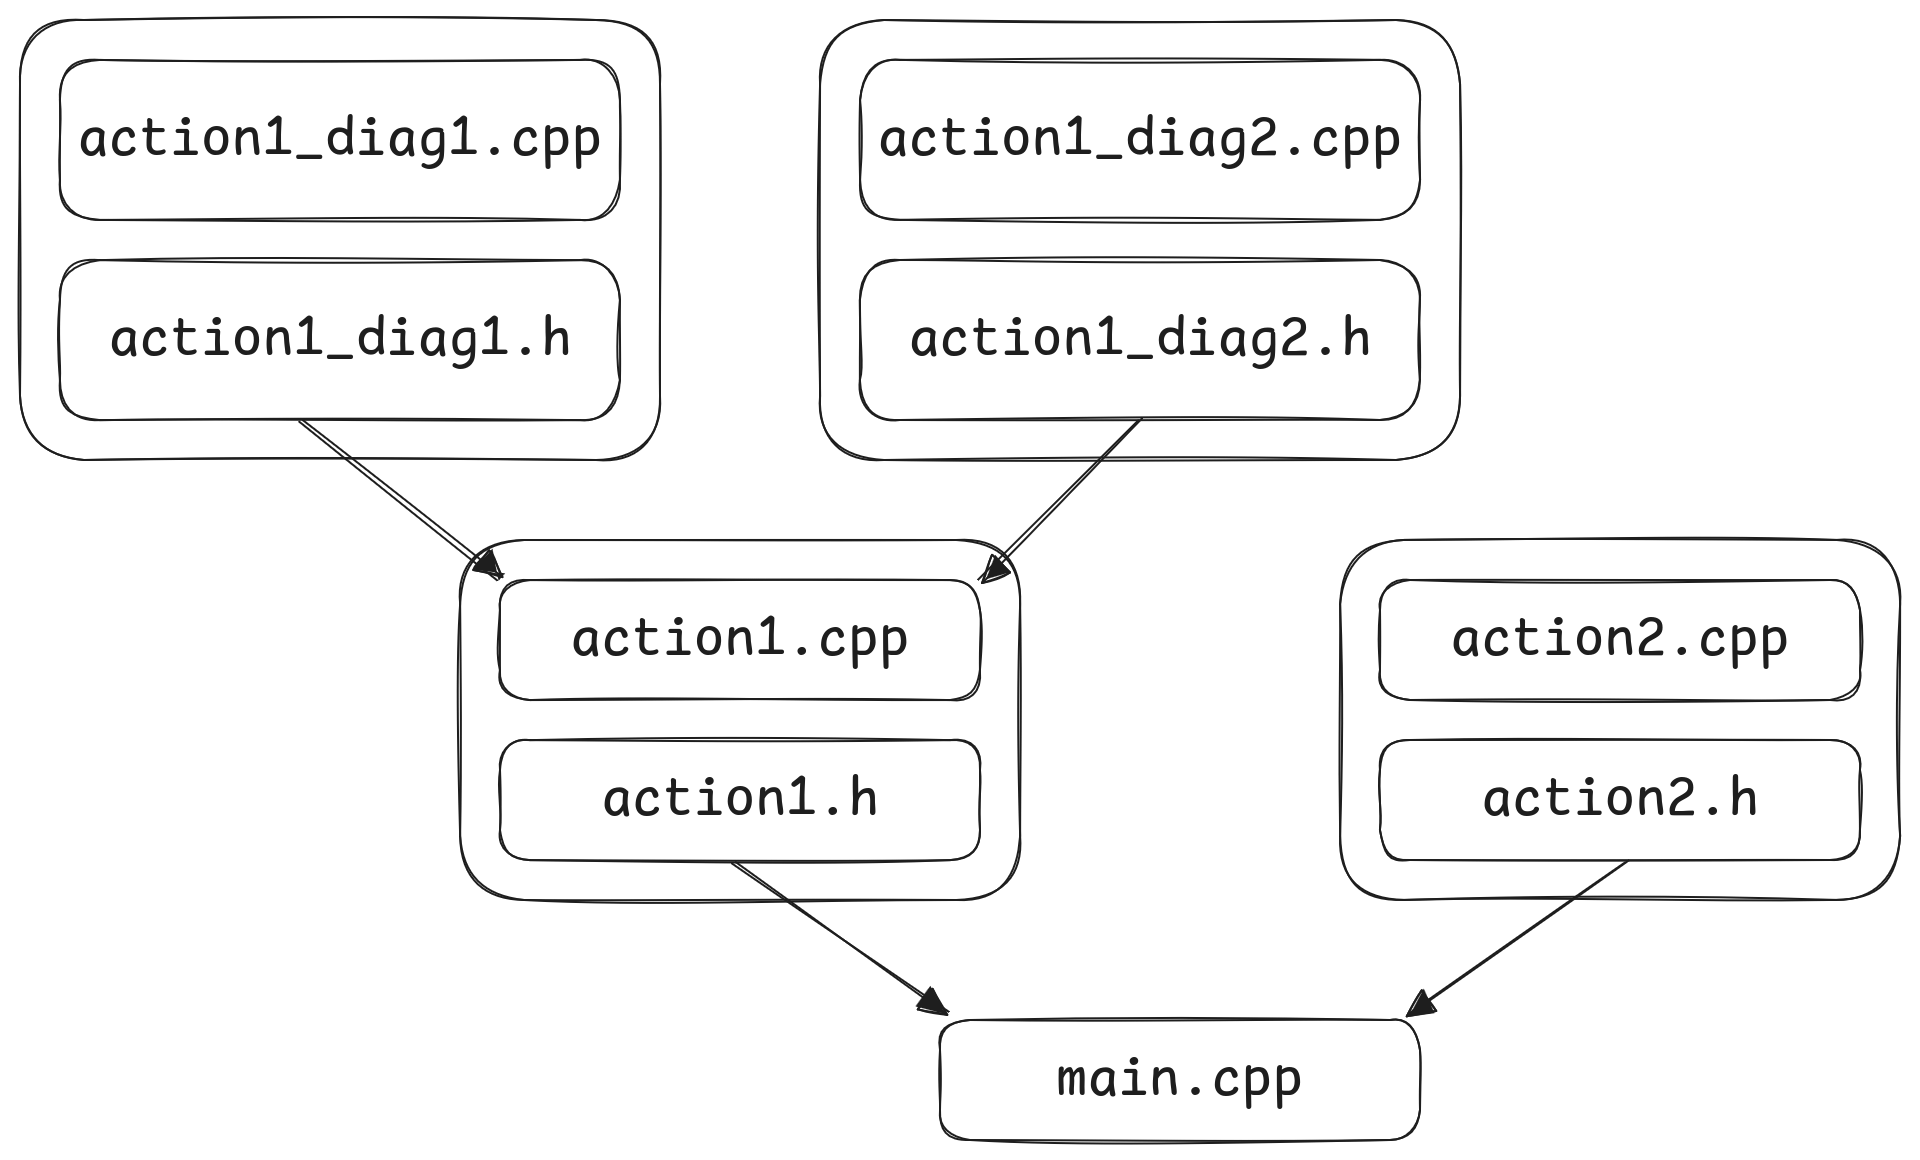
\includegraphics[width=0.7\linewidth]{include_diagram.png}
	\caption{\#include-ієрархія}
\end{figure}
\begin{figure}[p]
  \center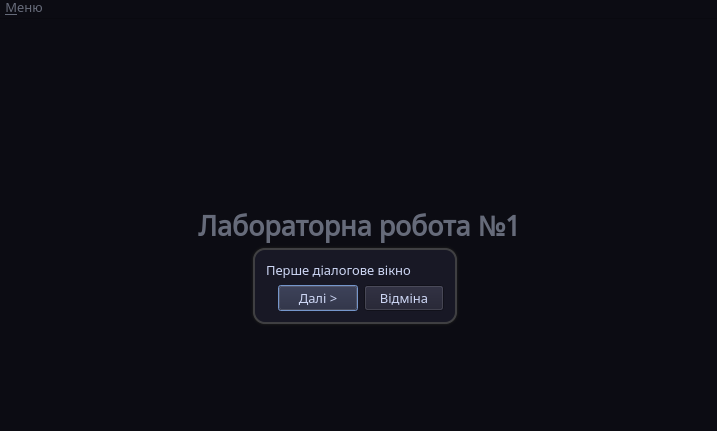
\includegraphics[width=0.7\linewidth]{action1_diag1.png}
	\caption{Робота 1: Перший діалог}
\end{figure}
\begin{figure}[p]
  \center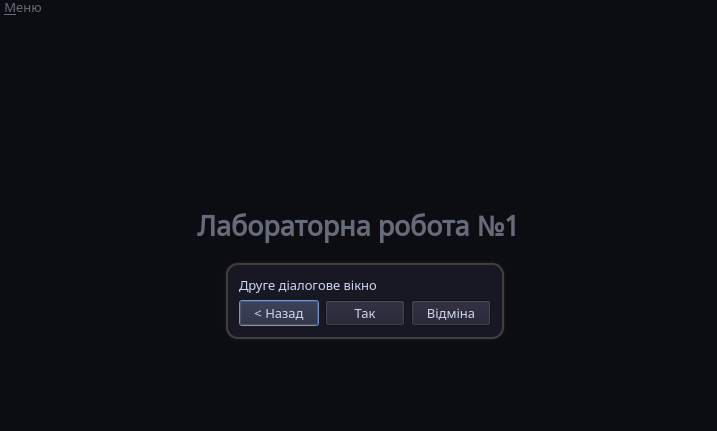
\includegraphics[width=0.7\linewidth]{action1_diag2.png}
	\caption{Робота 1: Другий діалог}
\end{figure}
\begin{figure}[p]
  \center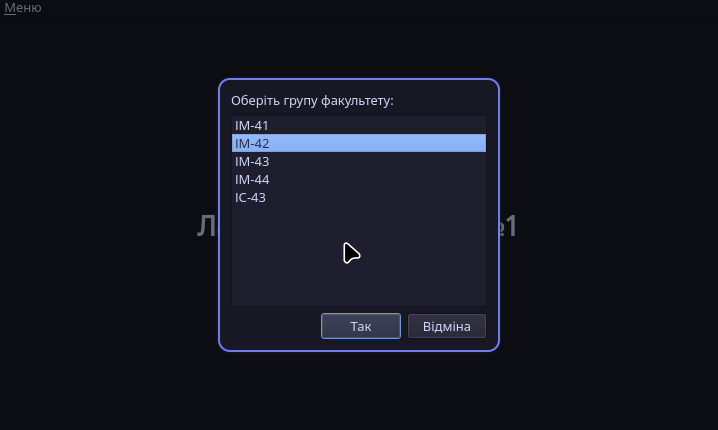
\includegraphics[width=0.7\linewidth]{action2_diag.png}
	\caption{Робота 2: Діалог}
\end{figure}
\begin{figure}[pt]
  \center
\includegraphics[width=0.7\linewidth]{action2_result.png}
	\caption{Робота 2: Результат}
\end{figure}

\pagebreak

\conclusion%
Написав графічний застосунок за допомогою фреймворку Qt6.
Розділив логіку виконання роботи на модулі так, що кожен модуль містить певну
логіку відображення одного діалогового вікна (або групи вікон). Водночас,
переконався, щоб дерево залежностей було направлене строго у напрямку до
головного виконуваного файлу.
\end{document}

% vim: ts=2: sw=2
